\documentclass[11pt, a4paper]{article}
\usepackage[margin=2.5cm]{geometry}
\usepackage{parskip}
\usepackage{booktabs}
\usepackage{hyperref}
\usepackage{amsmath}
\usepackage{xcolor}
\usepackage{graphicx}
\usepackage{float}
\usepackage{caption}
\captionsetup{font = footnotesize}
\usepackage{natbib} 
\definecolor{noteblue}{RGB}{30, 90, 160}

\title{\textbf{Manuscript Outline}\\
\large Climate and the molecular evolution of Influenza A surface proteins}
\author{Nina Pust}
\date{\today}

\begin{document}
\maketitle

% ─────────────────────────────────────────────────────────────────────────────
\section*{Introduction}

%\subsection*{Influenza A epidemiology and climate}
Influenza A infections display marked seasonal patterns, peaking in winter months in temperate regions and in rainy seasons in the tropics (\cite{petrova_evolution_2018}), also causing devastating epidemics and most of the major pandemics in the last century (\cite{hsieh_influenza_2006, trovao_when_2020}). Local climates are likely to be involved in variant emergence by influencing mode of transmission, host immunity and respiratory tract conditions (\cite{kudo_low_2019}). Climatic conditions that allow greater droplet stability can relac the population bottleneck at transmission (\cite{frise_contact_2016}), reducing the loss of novel variants during host-to-host spread. Experimental work has shown that colder and dried conditions increase transmission efficiency due to enhanced virus survival in airborne droplets (\cite{lowen_influenza_2007, shaman_absolute_2009}). Meanwhile, hot and humid conditions might also promote viral survival by reducing dessication (\cite{minhaz_ud-dean_structural_2010}), such that the role of climate on variant emergence is likely complex (\cite{deyle_global_2016}) and remains poorly understood. Modern global-scale surveillance data frequently includes genetic sequences for the core hemagglutinin (HA) and neuraminidase (NA) viral surface protein genes, which provide fundamental information about strain emergence in addition to date and location of collection, even in the abselnce of additional patient information (\cite{volz_viral_2013}).  

The influenza viral surface proteins HA and NA are fast-evolving and directly involved in transmission and infection efficiency (\cite{nelson_evolution_2007}). HA binds to sialic acid on host glycoproteins or glycolipids, facilitationg viral entry into the host cell. Meanwhile, NA cleaves sialic acids on host and virion glycoproteins, enabling the release of virions from the host cells (\cite{matsuoka_comprehensive_2013}). The function od both od these surface proteins can be acutely affected by extracellular environmental conditions, in particular pH (\cite{klenow_influenza_2023, tosheva_hemagglutinin_2023}), pointing to strong selection pressures prior to cell access. Variants that require a lower pH for the activation of HA are thought to have a selective advantage in transmission, as they are less susceptible to inactivation in mildly acidic extracellular environments (\cite{russier_molecular_2016, singanayagam_influenza_2019, tosheva_hemagglutinin_2023}). Meanwhile, colder and drier conditions reduce mucus transport velocity (\cite{kelly_rapid_2021, kilgour_mucociliary_2004}) and likely pH in airways (\cite{kullmann_environmental_2008}). 

Dry air additionally impairs innate antiviral defence and tissue repair in mice, making regions with driest climates likely to worsen susceptibility to severe disease (\cite{kudo_low_2019}) . Environmental temperature and humidity might therefore impact viral evolution via either changed infection times, viral loads, and selection pressures mediated by factors like airway mucus composition. Alternatively, outdoor environmental climate might not be relecant predictor of viral novelty. This might occur if evolution is dominated by intracellular environment (\cite{partlow_influenza_2025}) or by demographic patterns of transmission driven by social habits and networks (\cite{cauchemez_role_2011, endo_within_2021}). 

In RNA viruses like influenza A, mutational genetic change, known as antigenic drift, is shaped by multiple factors including mutation rates, replication dynamics, and host immune pressures (\cite{nelson_evolution_2007, wille_ecology_2020}). Antigenic drift, influenced by host immunity and vaccination, is a potent driver of novel strain emergence in influenza (\cite{bedford_integrating_2014}), along with reassortment events between co-occurring lineages (i.e., antigenic shift) (\cite{nelson_evolution_2007}). Additionally, antigenic drift reduces vaccine eddicacy and maintains some regions as global virus reservoirs (\cite{naeem_antigenic_2020}). Environmental conditions can influenxe evolutionary rates either directly via physical conditions for virion survival, or indirectly by altering social dynamics and people movement. Global climate change might therefore alter the prevalebce and geographic distribution of evolutionary hotspots, likely causing more recurrent or ongoing outbreaks compared to the seasonal peaks currently observed in temperate regions (\cite{baker_implications_2021}). Such changes elevate the risk of novel strain emergence, underscoring the need to test the importance of climate for viral evolution. 

In this study, we use a global data set of influenza A to test for the links between local climate, population density, and rates of molecular evolution of surface antigens in two most common seasonal strains; H1N1 and H3N2. Additionally, we use the polymerase acidic protein gene (PA), an internal, slow-evolving gene, as a negative control. Using a dataset with over \textbf{[X]} surveillance samples of each of the genes, sampled globally across two strains, we inferred terminal branch rates and non-synonymous and synonymous substitution rates per sample. We then drew from global climatic and demographic databases to prepare a per-sample dataset of time-stamped temperature, humidity, and population density. Comparative analysis was then performed on these data to test for fundamental climatic or demographic predictors of evolutionary rates. By characterizing how climate influences viral evolutionary dynamics, we propose hypotheses for the formation of influenza A evolutionary hotspots and seasonal peaks under global climatic change.  

\section*{Results}

To asses whether local climate conditions shape influenza A evolution, we applied phylogenetic comparative regression to substitution rates estimated across H1N1 and H3N2 sequences spanning between 2009 and 2019 across 168 countries (Figure \ref{fig:main}A). Surface proteins HA and NA were tested due to their fast-evolving nature and key role in immune escape, while PA served as a negative control. 

To account for the confounding seasonal burden of influenza A infections in winter months, sampling density was added as a response. The results reveal that HA sequences collected at higher temperature show a decreased substitution rate (Figure \ref{fig:main}C). This effect was not observed in NA and PA. 

\begin{figure}[H]
  \centering
  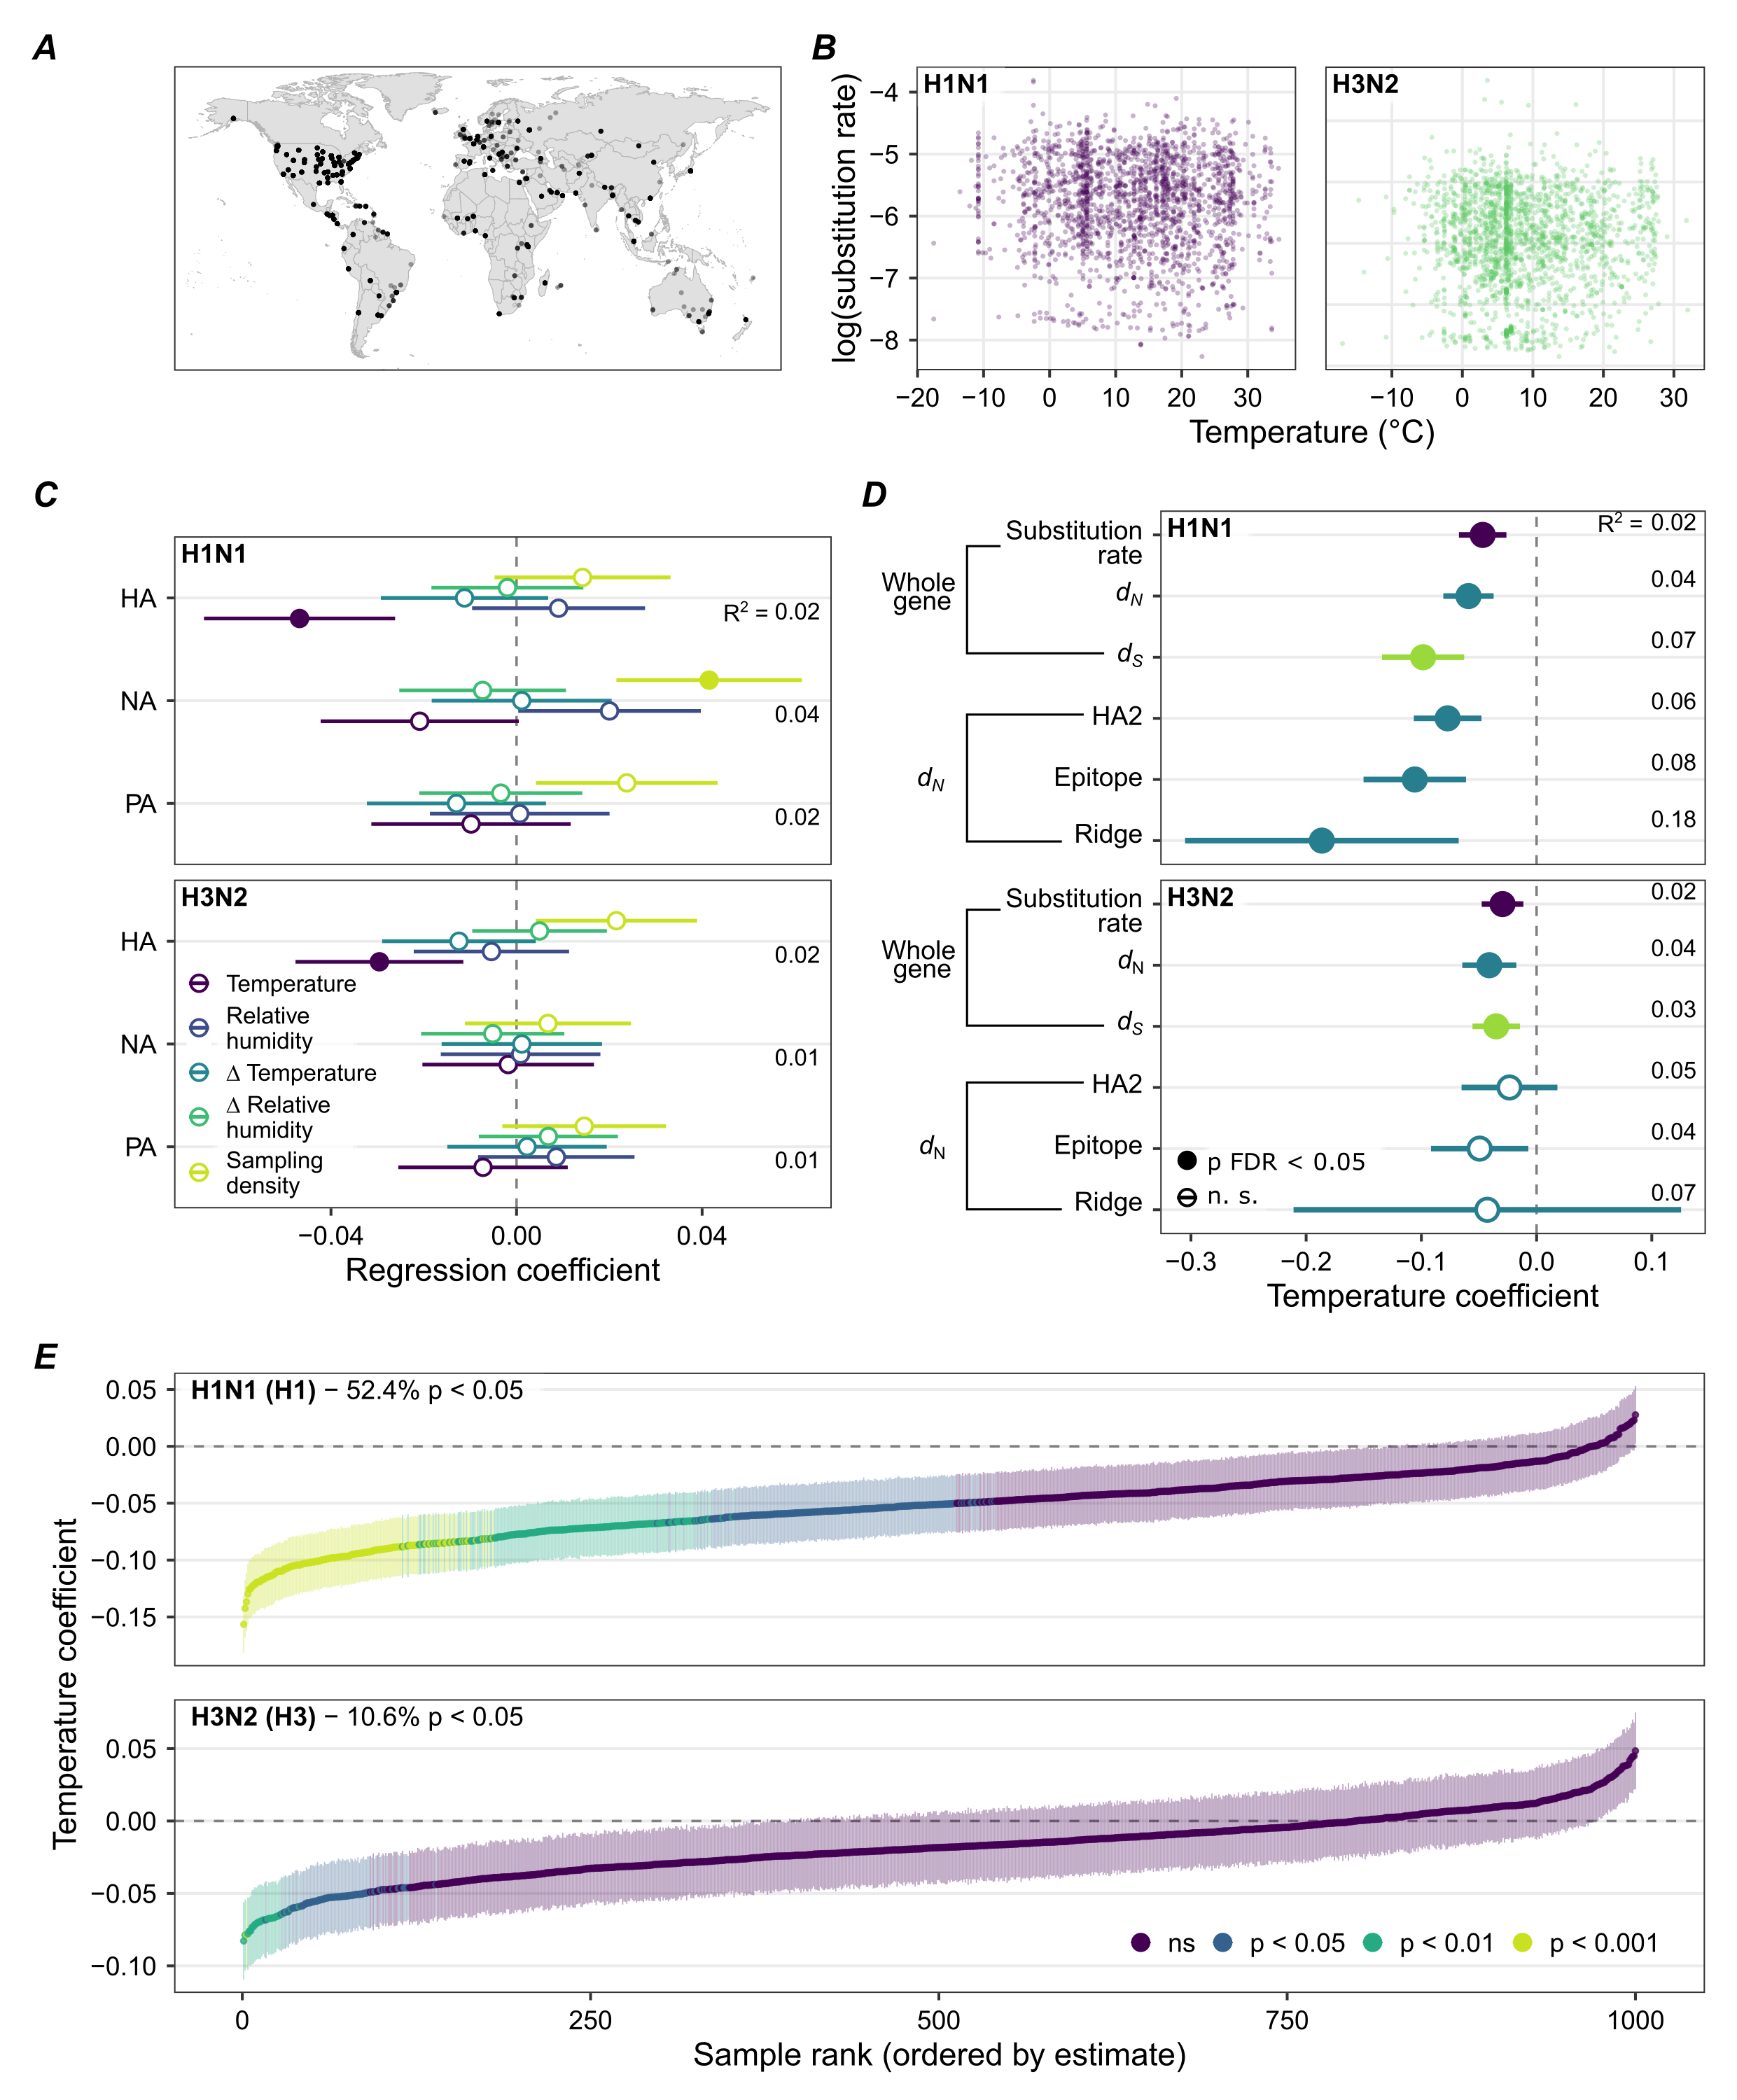
\includegraphics[width=\textwidth]{figures/fig1_mod.png}
  \caption{\textbf{(A)} Global distribution of H1N1 and H3N2 used in the analysis. \textbf{(B)} Overall substitution rate and temperature of each H1N1 and H3N2 sample used in the analysis. \textbf{(C)} Phylogenetic regression coefficients for the association between each climate predictor and the overall substitution rate with 95\% confidence intervals. Filled symbols indicate associations significant after Benjamini--Hochberg FDR correction ($p_{\text{FDR}} < 0.05$). \textbf{(D)} Regression coefficients for temperature specifically, split by antigenic ridge, broader epitope region, and stalk region (HA2). Filled symbols indicate FDR-significant associations. \textbf{(E)} Block jackknife sensitivity analysis: regression coefficients for temperature estimated after subsampling 1000 sequences from the dataset 1000 times, confirming that results are not driven by any single sequence or set of sequences.}
  \label{fig:main}
\end{figure}

To further look into the impact of temperature on HA substitution rate, the rate of synonymous ($d_{\text{S}}$) and non-synonymous ($d_{\text{N}}$) change was analysed on the whole gene, the stalk region (HA2), the epitope regions and the antigenic ridge (\textcolor{red}{Supp figure gene map}). No notable difference was observed between the $d_{\text{N}}$, $d_{\text{S}}$ and overall substitution rates across both analysed subtypes (Figure \ref{fig:main}D), implying that temperature plays a role in mutational rate, but doesn't influence selection. Analyses on the stalk region (HA2), epitope regions and the antigenic ridge showed that the temperature signal persists across gene regions of H1, while H3 does not reach significance on these analyses. This could be due to the reduced statistical power of only taking sequences that have undergone a non-synonymous change in each respective gene region, along with the fact that the overall regression analysis was less significant in H3N2 than in H1N1 ($p_{\text{FDR(H1N1)}} = value$, $p_{\text{FDR(H3N2)}} = value$). 

A similar trend can be observed in the block jackknife sensitivity analysis, showing that temperature has a significant negative effect on H1 in 52\% of subsamples with reduced statistical power, but only in 10\% in H3 (\ref{fig:main}E). Furthermore, this analysis revealed that the temperature signal was not driven by any particular sequence or set of sequences, but rather evenly distributed across the dataset (\textcolor{red}{Supp figure per sequence jackknives}). 

An in-depth analysis of non-synonymous mutations on the antigenic ridge and epitope regions of H1 and H3 revealed that several amino acid substitutions occur independently multiple times across taxa (Figure \ref{fig:mutations}, top row). However, a Wilcoxon rank-sum test reveals that no association between each substitution and each climate variable reaches statistical significance (Figure \ref{fig:mutations}, bottom row)
\begin{figure}[H]
  \centering
  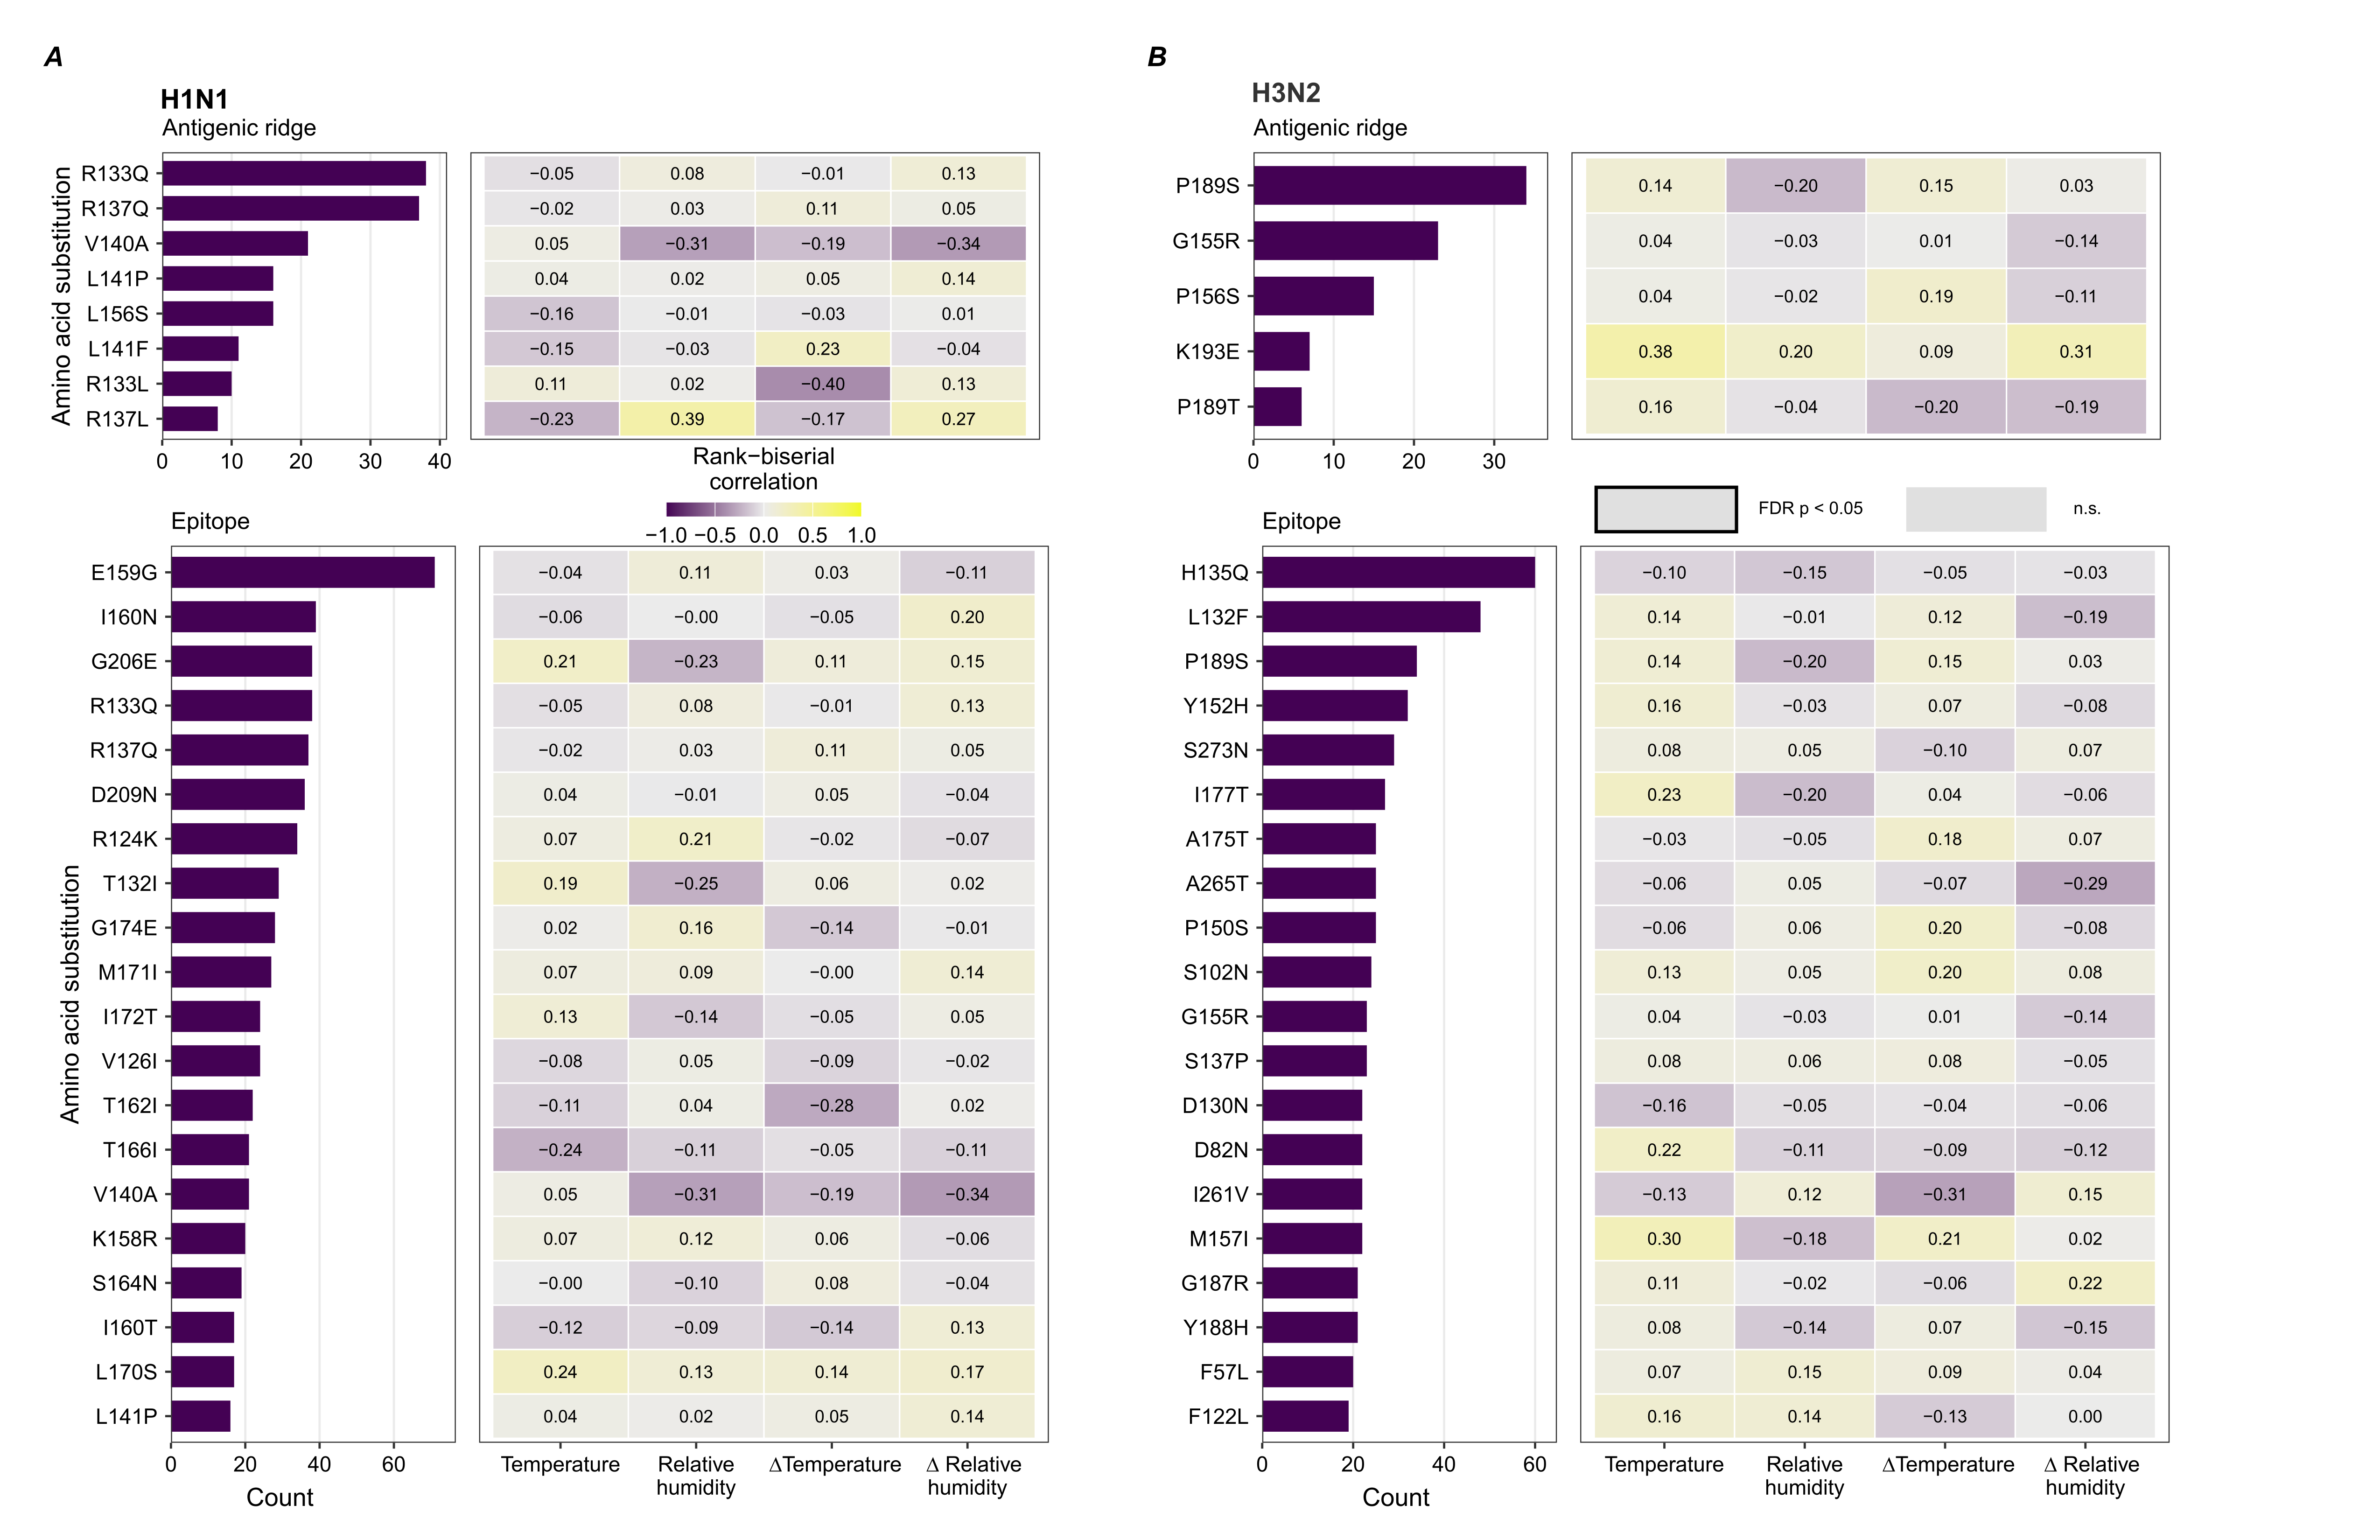
\includegraphics[width=\textwidth]{figures/fig2_mutations_mod.png}
  \caption{\textbf{Recurrent amino acid substitutions in the antigenic ridge and
    epitope regions do not show climate-specific enrichment.}
    Bar plots (left of each panel pair) show the number of independent
    evolutionary occurrences of each amino acid substitution (occurrences
    $> 5$) in the haemagglutinin antigenic ridge (top row) and
    the broader epitope region (bottom row) 20 most frequent
    substitutions shown) for H1N1 (\textbf{A}) and H3N2
    (\textbf{B}).
    Heatmaps (right of each panel pair) display the rank-biserial correlation
    between each climate variable (temperature, relative humidity, and their
    seasonal deltas) and the presence or absence of each substitution, estimated
    by a Wilcoxon rank-sum test.
    No substitution reaches statistical significance after Benjamini--Hochberg
    false discovery rate correction (FDR $< 0.05$; black tile border), indicating
    that climate does not selectively drive any specific amino acid change in the
    antigenic surface of HA.}
  \label{fig:mutations}
\end{figure}

\section*{Discussion}

\begin{itemize}

    \item \textbf{Restate the core finding and its novelty.}
    Open by briefly summarising what was found: a significant negative association between local temperature and HA substitution rate in both H1N1 and H3N2, robust to subsampling, not driven by any single sequence or outbreak cluster. Situate this in the literature — prior work has linked climate to influenza \emph{transmission}, but direct evidence linking ambient conditions to evolutionary rate in a global dataset is limited. This is the contribution.

    \item \textbf{Interpret the direction: cold $\rightarrow$ faster evolution.}
    Discuss that the direction is consistent with the well-established winter-season dominance in temperate regions. Cold conditions are associated with drier indoor air, longer outdoor aerosol persistence, reduced mucociliary clearance, and potentially lower airway pH — all of which may extend the transmission bottleneck window and expose a larger within-host viral population to selection. Faster replication cycles or larger effective population sizes at transmission could manifest as an elevated substitution rate at the population level even without a change in per-replication error rate.

    \item \textbf{Why both $d_\text{N}$ and $d_\text{S}$? Mutational rate, not altered selection.}
    The lack of a differential effect on $\omega$ ($d_\text{N}/d_\text{S}$) and the fact that the signal persists in synonymous as well as non-synonymous rates suggests that temperature is modulating the overall rate of molecular change rather than the \emph{type} of change (i.e.\ not shifting the balance of positive vs.\ purifying selection). A plausible interpretation is that colder, drier conditions lead to larger within-host population sizes or more replication rounds per transmission chain, generating more raw mutations — both synonymous and non-synonymous — without specifically enriching for adaptive change. This interpretation is also consistent with the mutation-frequency analysis showing no specific amino acid substitution enriched in colder climates.

    \item \textbf{Why HA and not NA or PA?}
    This is probably the most interesting question. HA is the primary target of humoral immunity and is under strong immune-driven positive selection, meaning it has the most headroom for variation. Possible explanations: (1) HA faces direct extracellular selection pressure (pH, mucus, antibody) that amplifies any climate-induced change in mutational supply; (2) NA evolves under different immune and functional constraints and may be subject to epistatic coupling with HA that buffers its rate; (3) the PA negative-control result confirms the pipeline is not generating spurious signals, and the NA null result is biologically informative rather than a power failure (NA sample sizes are comparable). Worth briefly considering whether the HA--climate link is HA-specific or just a consequence of HA evolving fastest overall (highest absolute rate), making small climate-linked differences easier to detect.

    \item \textbf{Why H1 more robustly than H3?}
    The subregion analyses and jackknife reach significance more consistently in H1N1 than H3N2. Discuss possible explanations: H3 HA is generally considered more antigenically variable and may evolve under stronger immune-driven directional selection that swamps a subtler climate signal; alternatively, H3N2 sampling is more geographically concentrated in certain years, potentially introducing confounders. The fact that the full-dataset association is nominally significant in both subtypes but the subregion analyses lose power in H3 is consistent with the signal being genuine but noisier — this should be presented as a caveat, not a contradiction.

    \item \textbf{What the recurrent-mutation analysis adds.}
    No specific substitution is enriched in colder/drier climates, despite several positions showing recurrent independent origins. This means climate is not deterministically channelling HA toward particular antigenic variants — it accelerates the overall clock without biasing the direction of change. Discuss what this implies for immune escape: more mutations per unit time increases the chance that a novel antigenic variant arises by chance, but climate does not directly select for any one epitope configuration.

    \item \textbf{Limitations.}
    (1) \emph{Ecological inference}: the climate predictor is the monthly mean at the collection site, which approximates the conditions experienced during transmission but not the within-host or indoor environment. (2) \emph{Surveillance bias}: GISAID submissions are heavily concentrated in North America, Europe, and East Asia — regions that are also the most climatically diverse in winter, which may inflate the apparent climate signal or create geographic confounders. Sampling density is included as a covariate to partially address this, but residual bias cannot be ruled out. (3) \emph{Temporal confounding}: collection year is controlled as a factor, but long-term evolutionary trends within subtypes (e.g.\ clade replacements) may not be fully accounted for. (4) \emph{Population density}: the GHSL-derived population density was included but deserves explicit discussion of its limitations (coarse resolution, static 5-year epochs vs.\ dynamic human movement). (5) \emph{Reverse causality is unlikely} but worth acknowledging: the global climate signal is contemporaneous with collection, not lagged, which weakens transmission-timing confounds.

    \item \textbf{Broader implications and future directions.}
    If cold, dry conditions accelerate HA evolution globally, regions undergoing climate change may experience shifts in the geographic distribution of evolutionary hotspots — potentially prolonging high-rate seasons in regions where winters are becoming shorter, or creating new hotspots in subtropical regions as humidity patterns shift. A logical extension of this work would be to incorporate within-country climate variation, lagged climate variables (reflecting the transmission chain prior to collection), and host population immunity data. Longitudinal modelling of how climate-associated rate changes translate to antigenic novelty and vaccine mismatch would be a high-impact follow-up.

\end{itemize}

Our results showed a significant negative association between hemagglutinin evolution and temperature, regardless of mutation type ($d_\text{N}$, $d_\text{S}$ ) in both H1N1 and H3N2 subtypes. Additionally, analyses on different regions of the H1 gene showed that temperature impacts both highly evolving regions (epitope, ridge) and slower evolving regions (stalk). No particular type of mutation in the epitope or antigenic ridge was associated with climate variables in any of the subtypes. Additionally, a sensitivity analysis showed that the signal persists even with a smaller sample size and isn't being driven by outlier sequences or particular outbreaks. We can therefore conclude that lower temperatures play a direct role in accelerating the rate of influenza A hemagglutinin evolution. No such effects were observed in NA genes or the negative control PA genes. 

\section*{Methods}

This analysis used a global sample of HA, NA and PA from H1N1 and H3N2 subtypes, collected between 2009-2019. Originally passaged sequences matching this criteria were obtained from GISAID EpiFlu along with their metadata detailing their location and collection date (\cite{shu_gisaid_2017}). Location strings found in the metadata were geocoded to latitude and longitude via Nominatim (OpenStreetMap) (\cite{noauthor_architecture_nodate, noauthor_openstreetmap_nodate}) with a hierarchical fallback to coarser geographic levels. For each date and location, a monthly mean temperature(2-m air) and 2-m dewpoint temperature was fetched from the Copernicus Climate Data Store at a $~0.1^\circ$ spatial resolution (\cite{noauthor_era5_nodate}). Relative humidity was derived from temperature and dewpoint using the Magnus formula. $\Delta\text{T}$ and $\Delta\text{RH}$ were computed as the difference between the collection month and the preceding month at the same location. Population density was extracted from the Global Human Settlement Layer (GHSL R2023A, 100m resolution, Mollweide projection) at the geocoded sample coordinates with the GHSL epoch (2010/2015/2020) matched to the sample collection year (\cite{pesaresi_advances_2024}). To control for uneven global surveillance effort, sampling density was computed as the count of sequences in the dataset sharing the same location and collection year and month. 

Sequences were aligned using MAFFT (\cite{katoh_mafft_2013}) and alignment columns with $>$50\% gaps were removed. Duplicated sequences were removed (Table \ref{tab:sequences}).  An initial maximum likelihood phylogeny was inferred with MAPLE v0.6.8 (\textcolor{red}{verify}) (\cite{de_maio_maximum_2022}) and time-calibrated with TreeTime using a relaxed clock and collection dates as calibrations (\cite{sagulenko_treetime_2018}). Sequences identified as clock outliers by TreeTime were excluded and a second MAPLE tree was inferred with the clock-filtered sequence set. The second round MAPLE tree was then time-calibrated with TreeTime once again, using the same relaxed clock. 


\begin{table}
    \centering
\caption{Number of sequences throughout the pipeline}
\label{tab:sequences}
    \begin{tabular}{cccccl}\toprule
         &  GISAID EpiFlu N&  After deduplication&  MAPLE tree round 2& Final &Retained [\%]\\\midrule
         H1&  17,519&  10,918&  10,913&  9,329&53.2\%\\
         N1&  18,225&  9,579&  9,571&  8,163&44.8\%\\
         PA (H1N1)&  14,289&  8,821&  8,819&  7,534&52.7\%\\
         H3&  25,594&  15,002&  15,000&  12,800&50.0\%\\
         N2&  25,586&  13,054&  13,053&  11,140&43.5\%\\
         PA (H3N2)&  22,407&  12,892&  12,890&  11,035&49.2\%\\ \bottomrule
    \end{tabular}
    
    
\end{table}

Pairwise synonymous ($d_\text{S}$) and non-synonymous ($d_\text{N}$) distances were estimated for all sequence pairs using yn00 (\cite{yang_estimating_2000}) implemented in PAML using F3$\times$4 codon frequencies and the standard genetic code. Codon columns containing stop codons or gaps were removed prior to each pairwise calculation. Per-sample mean $d_\text{N}$ and $d_\text{S}$ were computed as row means of the pairwise distance matrices. Samples with numerically unstable rates (log rate $< -$8) were removed (Table \ref{tab:sequences}, column 'Final'). 

To account for concentration of adaptive evolution of hemagglutinin in the antigenic surface sites (\textcolor{red}{insert citation}), the rate of non-synonymous change was analysed separately for the antigenic ridge, the broader epitope regions and the HA2 stalk region, used to infer whether the antigenic regions were driving the signal across the whole gene.  H1 sequence A/Puerto Rico/8/1934 CY009444 (\textcolor{red}{citation}) and H3 sequence A/Aichi/2/1968 CY12168 (\textcolor{red}{citation}) were used as references to map the positions of gene subregions (\textcolor{red}{Supp figure: gene maps}), which were then extracted from the full MAFFT alignment. For each tip, the ancestral codon at each position was inferred by maximum parsimony using phangorn (\cite{schliep_phangorn_2011}).  The tip codon was then compared to its inferred ancestor and classified as synonymous or non-synonymous. (\textcolor{red}{mention why we didn't use yn00 for this}). Stop codons, gaps, and ambiguous bases were excluded. The per-tip non-synonymous rate was calculated by dividing the count of non-synonymous changes with the time of the branch (\textcolor{red}{phrase this better}). Sequences not containing a non-synonymous change in the region undergoing analyses were removed. (\textcolor{red}{maybe have another table showing that}) 

Phylogenetic linear models were fitted with phylolm (\cite{ho_phylolm_2020}) while estimating Pagel's  $\lambda$
covariance. Analyses on the whole gene included two response variables: log overall evolutionary rate and log $\omega$, defined as  $\omega = d_\text{N} / d_\text{S}$. Analyses on the gene subregions used log non-synonymous substitution rate per subregion (antigenic ridge, epitope, HA2). Predictors used in all analyses were temperature [$^\circ$C], relative humidity [\%], $\Delta$-temperature, $\Delta$-humidity, sampling density (log-transformed), population density (log-transformed) and collection year as factor, controlling for secular trends. All phylolm results underwent Benjamini-Hochberg FDR corrections and associations with $p_\text{FDR} < 0.05$ were considered significant. 

Recurrent non-synonymous mutations (independent occurrences $>$ 5) were tested for association with each climate variable using the Wilcoxon rank-sum test. The effect size was quantified as the rank-biserial correlation. Benjamini-Hochberg FDR correction was applied within each gene and region. 

To asses whether the temperature association was robust to subsampling, a block jackknife was performed: 1000 year-stratified random subsamples of 1000 sequences (or, in the subregion cases, where N dropped below 1000, at 60\% of N) were drawn. The tree was pruned to each subsample and phylolm was refitted using a reduced formula where log substitution rate or non-synonymous rate (in the case of subregion analyses) was used as a response variable and scaled temperature and collection year as factor were used as predictors. The distribution of temperature coefficients across the 1000 subsamples, and the proportion reaching $p<0.05$ were used to confirm that the full-model signal was not driven by any sequence or temporal cluster. 


\newpage

\bibliographystyle{plainnat}
\bibliography{references}
\end{document}
